
%(BEGIN_QUESTION)
% Copyright 2012, Tony R. Kuphaldt, released under the Creative Commons Attribution License (v 1.0)
% This means you may do almost anything with this work of mine, so long as you give me proper credit

Write the integral expression represented by the shaded area on this graph (assuming each horizontal and vertical division on the graph has an incremental value of 1).  The integral for this shaded area has a {\it negative} value:

$$\includegraphics[width=15.5cm]{i01905x01.eps}$$

\underbar{file i01905}
%(END_QUESTION)





%(BEGIN_ANSWER)

There are two different ways to write this integral:

$$\int_{7}^{2.5} (8 - y) \> dx$$

$$\int_{2.5}^{7} (y - 8) \> dx$$

%(END_ANSWER)





%(BEGIN_NOTES)


%INDEX% Mathematics, calculus: integral (defined in a graphical sense)

%(END_NOTES)


